\documentclass{beamer}
\usepackage{graphicx}
\usepackage{amsmath,amsfonts,amssymb}
%exclude navigation symbols
\beamertemplatenavigationsymbolsempty
%\usetheme[compress]{default}
\usecolortheme{seagull}
\usefonttheme{structurebold}
\expandafter\def\expandafter\insertshorttitle\expandafter{\insertshorttitle\hfill\insertframenumber\,/\,\inserttotalframenumber}
\title[The RNA Workbench]{The RNA Workbench - reproducible, transparent, and accessible RNA research}
\author[RNA Workbench Team]{Florian Eggenhofer, Bj\"orn Gr\"uning, B\'{e}r\'{e}nice Batut, J\"org Fallmann, Andrea Bagnacani, Peter F. Stadler, Rolf Backofen and the RNA Workbench Team}
\institute[Bioinf]{Lehrstuhl Bioinformatik\\University of Freiburg}
\date{30.06.2017}
\subject{}
\keywords{}

\newcommand{\backupbegin}{
   \newcounter{finalframe}
   \setcounter{finalframe}{\value{framenumber}}
}
\newcommand{\backupend}{
   \setcounter{framenumber}{\value{finalframe}}
}

%\newcommand{\TODO}[1]{{\color{red} #1}}
\defbeamertemplate{footline}{higher page number}
{%
  \hfill%
  \usebeamercolor[fg]{page number in head/foot}%
  \usebeamerfont{page number in head/foot}%
  \raisebox{0.2cm}[0pt][0pt]{
  \insertframenumber\,/\,\inserttotalframenumber\kern1em}%
}
\setbeamertemplate{footline}[higher page number]
\begin{document}
\frame{
  \titlepage
}

\frame{
  \frametitle{Goals of the RNA Workbench}
  %Differences to previous work
  %\onslide<1->
  \begin{figure}
    \only<1>{
\includegraphics[width=0.5\textwidth]{figures/welcome_image_1.eps}}
    \only<2>{\hspace{-3.5pt}
\includegraphics[width=0.5\textwidth]{figures/welcome_image_2.eps}}
    \only<3>{\hspace{-7pt}
\includegraphics[width=0.5\textwidth]{figures/welcome_image_3.eps}}
    \only<4>{\hspace{-10.5pt}
\includegraphics[width=0.5\textwidth]{figures/welcome_image_4.eps}}
    \only<5>{\hspace{-14pt}
\includegraphics[width=0.5\textwidth]{figures/welcome_image_5.eps}}
    \only<6>{\hspace{-14pt}
\includegraphics[width=0.5\textwidth]{figures/welcome_image.eps}}
  \end{figure}
  \begin{itemize}
  \item<2-> Comprehensive set of \textit{RNA}-bioinformatics tools
  \item<3-> Community - authors and users
  \item<4-> Set of predefined workflows and associated descriptions/training material
  \item<5-> Easy and stable dissemination via Galaxy \onslide<6->{and Docker}
  \end{itemize}
}

\frame{
  \frametitle{Tools}
  %Tool logo cloud with categories
  \begin{itemize}
  \item More than 50 \textit{RNA} bioinformatics tools
  \item Classical RNA bioinformatics (INFERNAL, ViennaRNA, ..)
  \item RNA-seq analysis (FuMa, Paralizer, ..)
  \item Auxiliary tools - Visualisation
  \end{itemize}  
}


\frame{
  \frametitle{Workflows}
  \begin{itemize}
  \item Standardized analysis procedures
  \item Based on tools as building blocks
  \item Can be designed and shared (ToolShed/myexperiment.org)
  \item Currently six workflows %TODO - add workflows
  \end{itemize}
    %Turning history into workflow / design from scratch
  \begin{figure}
    \centering
    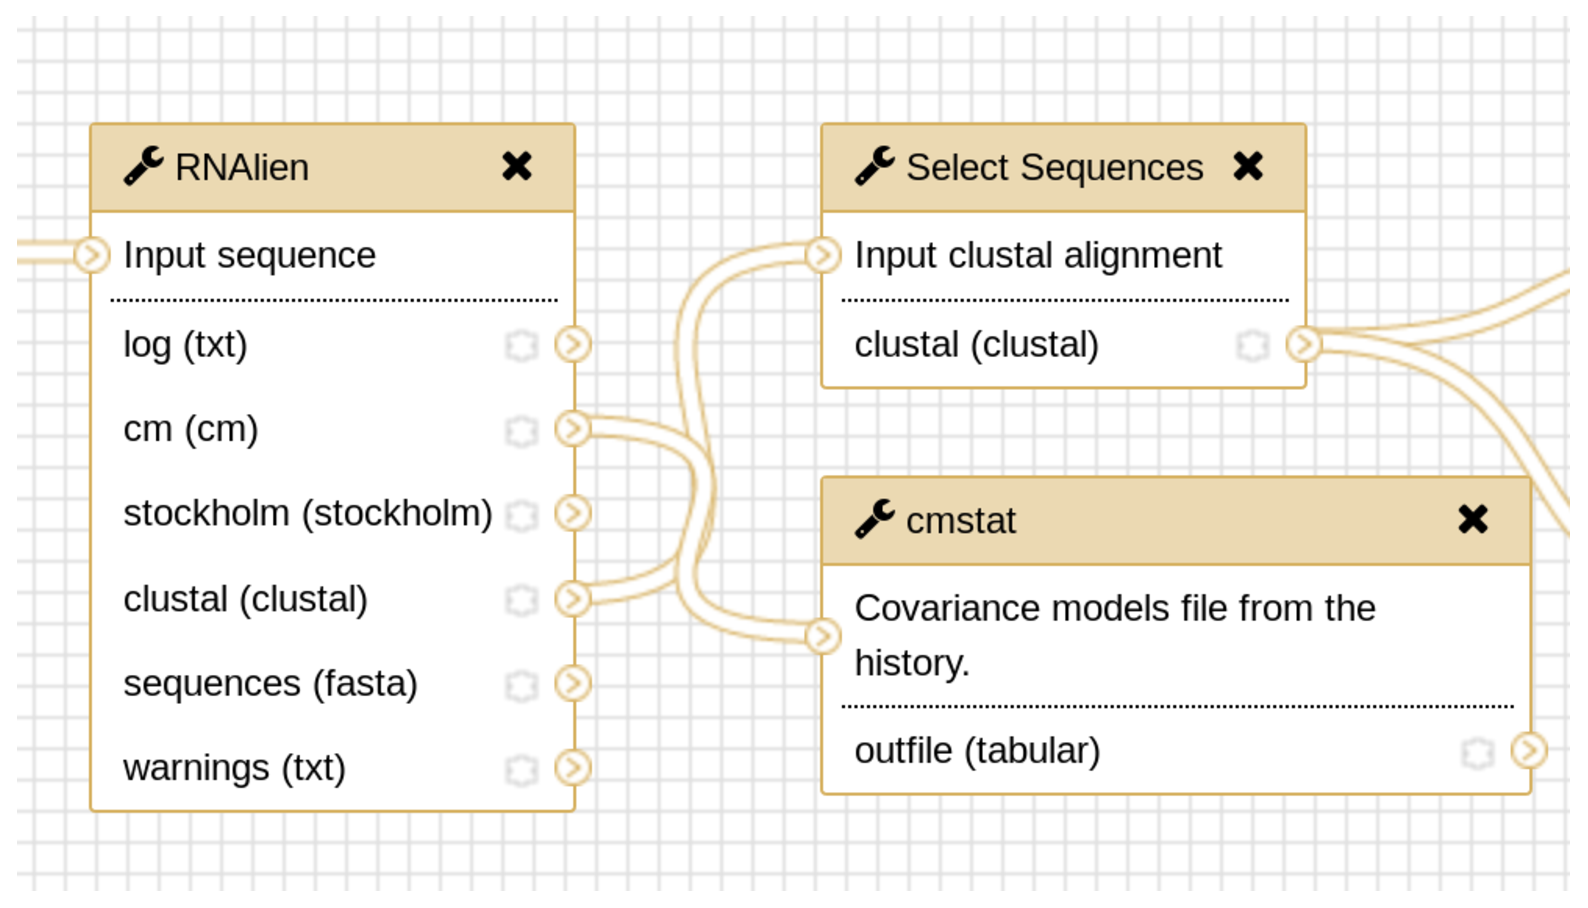
\includegraphics[width=0.5\textwidth]{figures/workflowdesign.eps}
  \end{figure}
}

\frame{
  \frametitle{Workflow - Analysis of non-coding \textit{RNA}s}
  \begin{itemize}
  \item Test for functional structure via conservation
  \end{itemize}
   \begin{figure}
     \centering
    \only<1>{
\includegraphics[width=0.8\textwidth]{figures/ncRNA_general_Workflow_1.eps}} 
    \only<2>{
\includegraphics[width=0.8\textwidth]{figures/ncRNA_general_Workflow_2.eps}}
    \only<3>{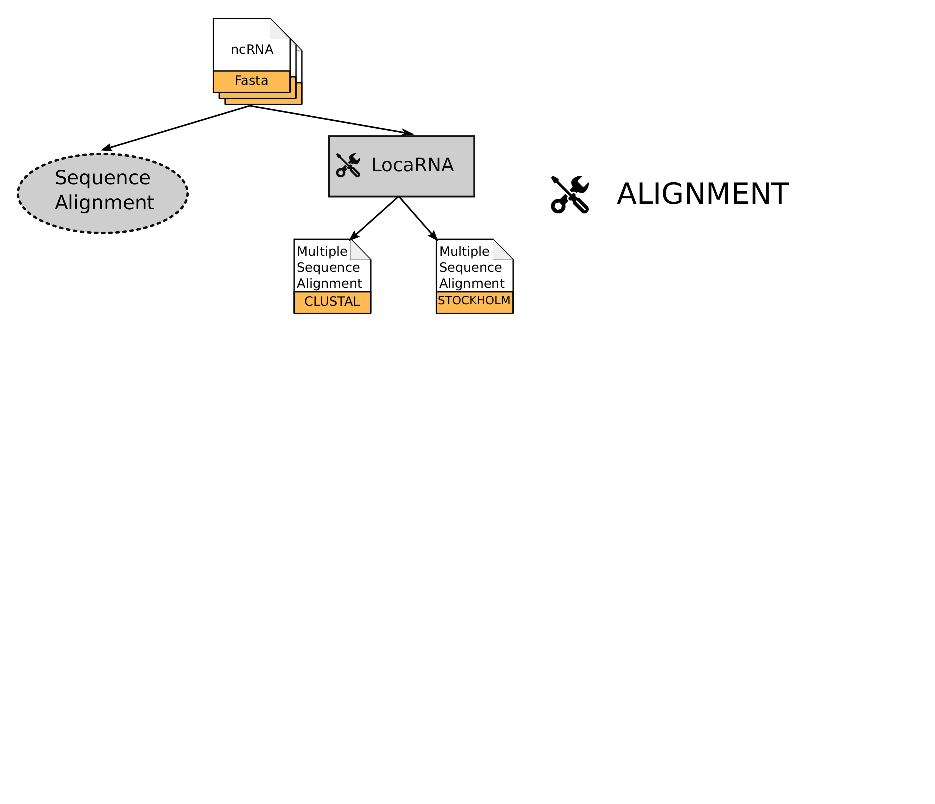
\includegraphics[width=0.8\textwidth]{figures/ncRNA_general_Workflow_3.eps}}
    \only<4>{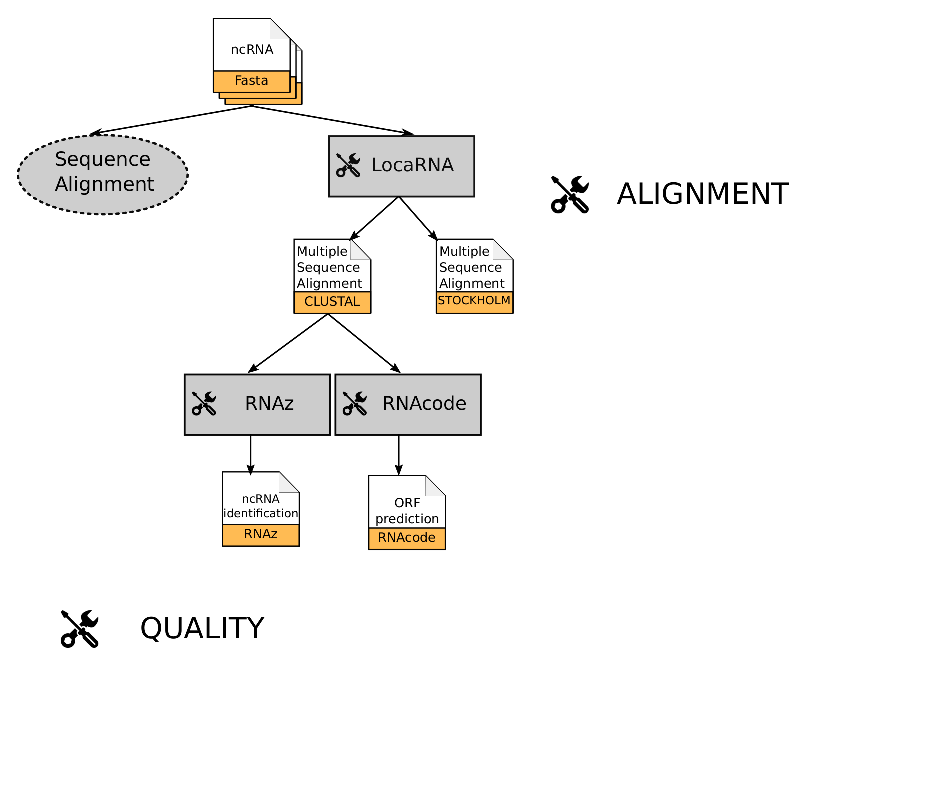
\includegraphics[width=0.8\textwidth]{figures/ncRNA_general_Workflow_4.eps}}
    \only<5>{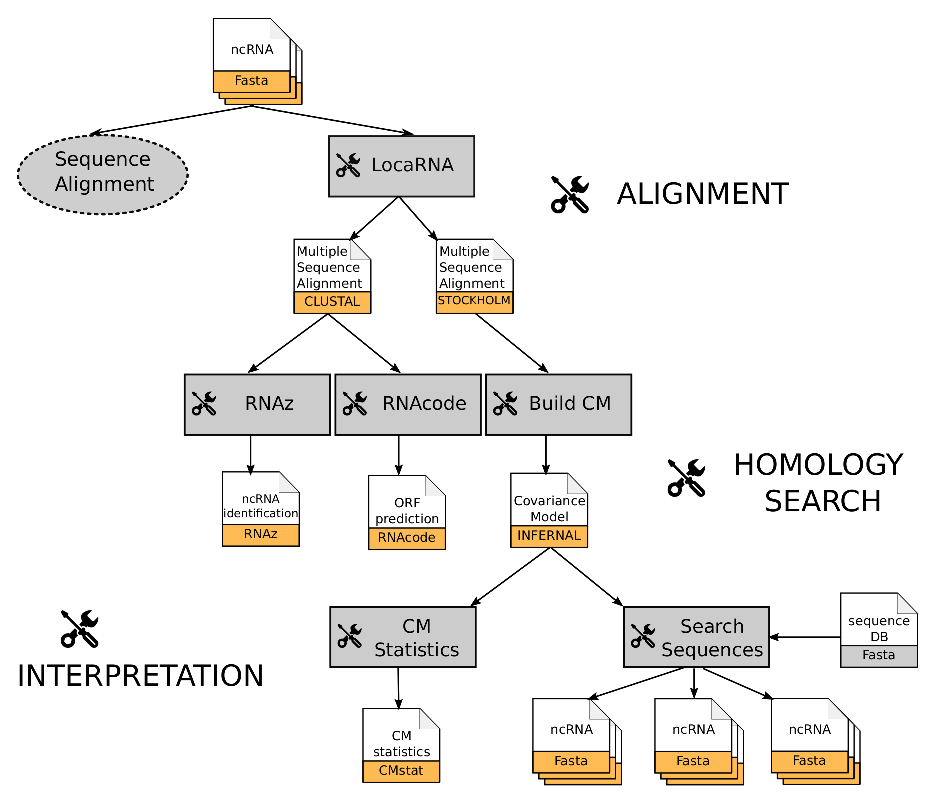
\includegraphics[width=0.8\textwidth]{figures/ncRNA_general_Workflow_5.eps}}
    %TODO add tools slide
  \end{figure}
  
}

\frame{
  \frametitle{Workflow - \textit{RNA} family model construction}
  \begin{itemize}
  \item RNA family model construction
  \end{itemize}
   \begin{figure}
     \centering
    \only<1>{
\includegraphics[width=0.8\textwidth]{figures/modelconstruction_Workflow1.eps}}
    \only<2>{
\includegraphics[width=0.8\textwidth]{figures/modelconstruction_Workflow2.eps}}
    \only<3>{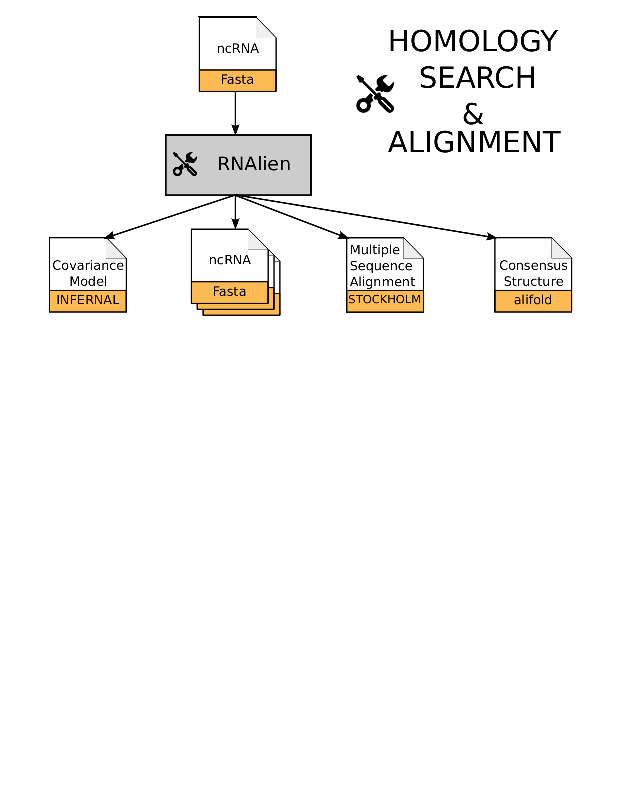
\includegraphics[width=0.8\textwidth]{figures/modelconstruction_Workflow3.eps}}
    \only<4>{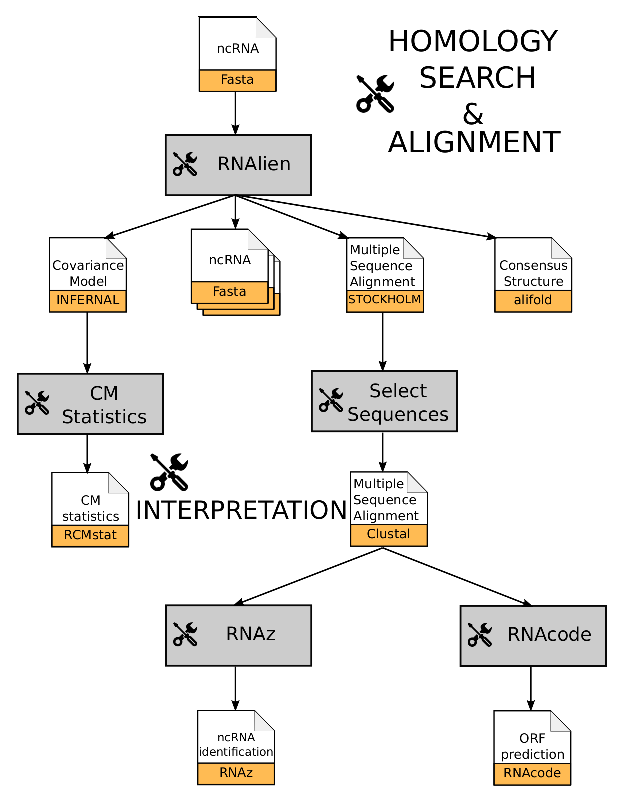
\includegraphics[width=0.8\textwidth]{figures/modelconstruction_Workflow4.eps}}
  \end{figure}
}


\frame{
  \frametitle{Implementation}
  \begin{itemize}
  \item Galaxy framework - reproducibility, usability %Accessiblility - webservice
  \item Docker - deployment, layers (Data, Tours, Documentation) %Workflows, Tools
    %layer figure?
  \item Bioconda - version management, dependencies % staying up-to-date
  \item Continious integration (CI) - testing
  \end{itemize}
  %using the workbench
  \begin{itemize}
  \item docker run -d -p 8080:80 bgruening/galaxy-rna-workbench
  \item OSX and Windows using the graphical tool Kitematic 
  \end{itemize}  
}

\frame{
  \frametitle{Training}
  \begin{itemize}
  \item Training sessions (Introduction, HTS data and \textit{RNA}-seq analyses)
  \item http://galaxyproject.github.io/training-material
  \item Galaxy Interactive Tours
  \end{itemize}  
}

\frame{
  \frametitle{Visualisation}
  \begin{itemize}
  \item General purpose bar chart scatter plot
  \item Connection to IGV, UCSC genome browsers
  \item Specific \textit{RNA} visualisation Dot plot, dot-bracket, tertiary structure (3D)
  \end{itemize}  
}


%\frame{
%  \frametitle{Using the workbench}
%  \begin{itemize}
%  \item docker run -d -p 8080:80 bgruening/galaxy-rna-workbench
%  \item OSX and Windows using the graphical tool Kitematic 
%  \end{itemize}  
%}


\frame{
  \frametitle{Community}
  \begin{itemize}
  \item Tool authors, galaxy developers and users
  \item Open participation, reward, and inclusion
  \item Galaxy, BioConda, BioContainers and BioJS
  \item GitHub, IRC, and Gitter
  \end{itemize}  
}


\frame{
  \frametitle{Acknowledgements \& Thanks}
  
\includegraphics[width=1\textwidth]{figures/funding.eps}
}

\frame{
  \frametitle{RNA-seq analysis: trimming, mapping and read count}
  \begin{itemize}
  \item Test for differential gene expression
  \item Quality control - Mapping \& Annotation - Differential expression
  \item Template for customized workflows
  \end{itemize}
  %Workflow Figure
}
\end{document}
